\ylDisplay{Killud} % Ülesande nimi
{Jaan Kalda} % Autor
{lahtine} % Voor
{2012} % Aasta
{G 10} % Ülesanne nr.
{9} % Raskustase
{
% Teema: Dünaamika
\ifStatement
Savikuulike massiga \SI{10}{g} kukkus vertikaalselt alla siledale horisontaalsele
põrandale ja läks kolmeks killuks.
Killud lendasid laiali ja peatusid punktides, mis on näidatud juuresoleval
joonisel
(ülaltvaade, ristiga on märgitud kukkumiskoht). Määrake kildude massid.
Joonisel (lisalehel)
võib teha lisakonstruktsioone ja mõõtmisi.
Võite lugeda, et killud hakkasid kohe pärast kukkumist üles põrkumata libisema,
õhuhõõre on tühine ja liugehõõrdetegur ei sõltu kiirusest.
\begin{center}
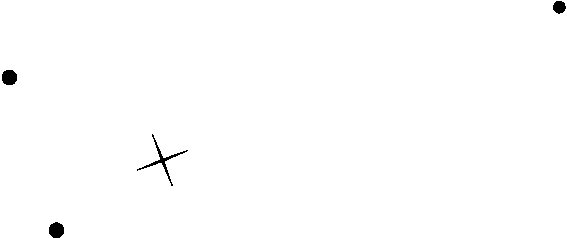
\includegraphics[width=0.8\linewidth]{2012-lahg-10-killud}
\end{center}
\fi


\ifHint
Kildude koguimpulss on null, seega moodustavad impulsivektorid kolmnurga, mille sarnasustegurid on võimalik kildude liikumissuundadest taastada. Sarnaselt saab toimida kildude kineetilise energia ja libisemiskaugustega.
\fi


\ifSolution
Kildude koguimpulss on null, seega moodustavad impulsivektorid kolmnurga, mille saame sarnasusteguri täpsusega taastada kildude liikumissuundade abil.
Sellest kolmnurgast saame küljepikkuste suhete mõõtmise abil teada algimpulsside suhted $p_1 : p_2: p_3 = \num{72} : \num{24} : \num{59}$ (need numbrid on 
kolmnurga külgede pikkused millimeetrites). 
Kildude libisemiskaugused suhtuvad kui algkiiruste ruudud --- mõõtmiste abil saame teada 
\[
v_1^2:v_2^2:v_3^2 = \num{72}:\num{30}:\num{21}
\]
ning ruutjuure võtmise järel ka 
kiiruste suhted
\[
v_1 : v_2: v_3 = \num{8,5}:\num{5,5}:\num{4,6}.
\]
Jagades impulsside suhted kiiruste suhtega, saame teada masside suhted
\[
m_1:m_2:m_3=\num{8,5}:\num{4,4}:\num{12,8}
\]
ning teades kogumassi ka massid eraldi võetuna,
\[
m_1=\SI {10}g\cdot \frac{\num{8,5}}{\num{8,5}+\num{4,4}+\num{12,8}} = \SI{3,3}g\text{, }m_2=\SI {10}g\cdot \frac{\num{4,4}}{\num{25,7}}=\SI{1,7}g\text{, } 
m_3=\SI {10}g\cdot \frac{\num{12,8}}{\num{25,7}}=\SI{5,0}g.
\]
\hspace*{0\columnwidth}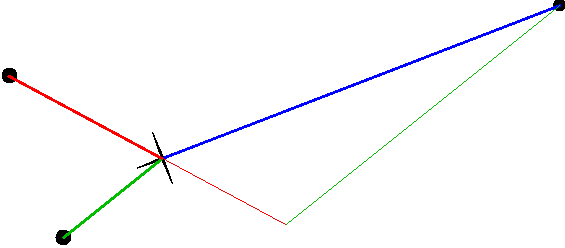
\includegraphics[width=\columnwidth]{2012-lahg-10-killud_lah}
\fi


\ifEngStatement
% Problem name: Fragments
A clay ball of mass 10 g fell vertically down to a smooth horizontal ground and broke into three fragments. The fragments scattered on the ground and stopped at points that are given in the figure (top view, the cross represents the falling point). Find the masses of the fragments. You can make additional designs on the drawing (on a separate paper) and take additional measurements. You can assume that the fragments started to slide right after the fall without bouncing upwards, the air friction is insignificant and that the coefficient of kinetic friction does not depend on the speed. 
\begin{center}
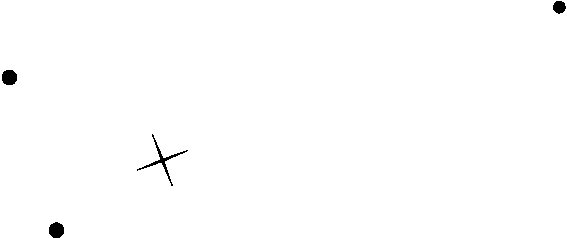
\includegraphics[width=0.8\linewidth]{2012-lahg-10-killud}
\end{center}
\fi


\ifEngHint
The total momentum of the fragments is zero, thus the vectors of momentum make up a triangle. Its similarity ratio can be restored from the movement directions of the fragments. You can act similarly with the kinetic energy and the sliding distances of the fragments.
\fi


\ifEngSolution
The total momentum of the fragments is zero, therefore the momentum vectors form a triangle which we can restore with the accuracy of similarity ratio and with the help of the movement directions of the fragments. From this triangle we can get the ratios of initial momentums $p_1 : p_2: p_3 = \num{72} : \num{24} : \num{59}$ by measuring the ratios of the side lengths (these numbers are the side lengths of the triangle in millimeters). The sliding distances of the fragments are proportional to the initial velocities squared – by measuring we get $v_1^2:v_2^2:v_3^2 = \num{72}:\num{30}:\num{21}$ and after taking square root we get the ratios of the velocities as well $v_1 : v_2: v_3 = \num{8,5}:\num{5,5}:\num{4,6}$. Dividing the ratios of momentums with the ratio of velocities we get the ratios of masses $m_1:m_2:m_3=\num{8.5}:\num{4,4}:\num{12,8}$ and knowing the total mass we can find the masses separately $m_1=\SI {10}g\cdot \frac{\num{8,5}}{\num{8,5}+\num{4,4}+\num{12,8}} = \SI{3,3}g$, $m_2=\SI {10}g\cdot \frac{\num{4,4}}{\num{25,7}}=\SI{1,7}g$, $m_3=\SI {10}g\cdot \frac{\num{12,8}}{\num{25,7}}=\SI{5,0}g$.
\begin{center}
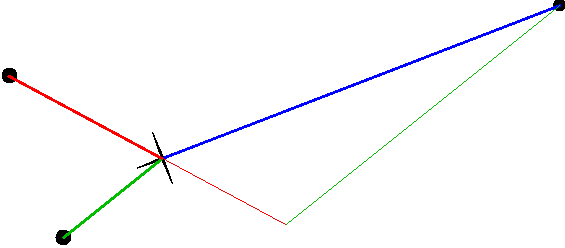
\includegraphics[width=\columnwidth]{2012-lahg-10-killud_lah}
\end{center}
\fi
}